TODO discuss choice of text size on smartphone

As the application launches, the first screen the user sees, in both versions, is the camera screen. The user must, in order to proceed further within the application, scan a QR code. Scanning a QR code is done by positioning the camera on the device (either Google Glass or smartphone) such that the QR code can be seen on screen. The user does not need to press any shutter button as the application automatically recognises the QR code pattern if seen on screen.%, as seen in Figure~\ref{}. The reasoning behind 

%	\begin{figure}[ht!]
%		\centering
%		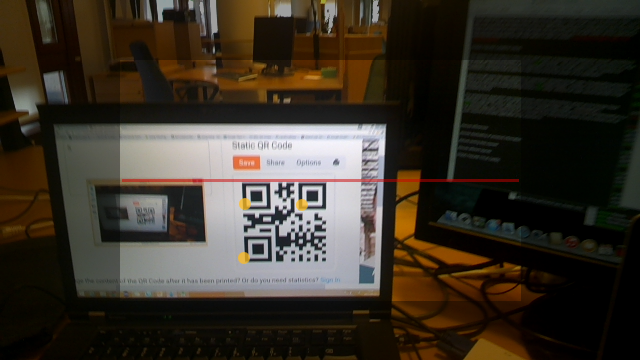
\includegraphics[width=110mm]{images/demo/qrCode}
%		\caption{todo bild behöver uppdateras}
%		\label{glassDemoQR}
%	\end{figure}
	
	\begin{figure}[ht!]
		\centering
    		\subfloat[The Google Glass application]{{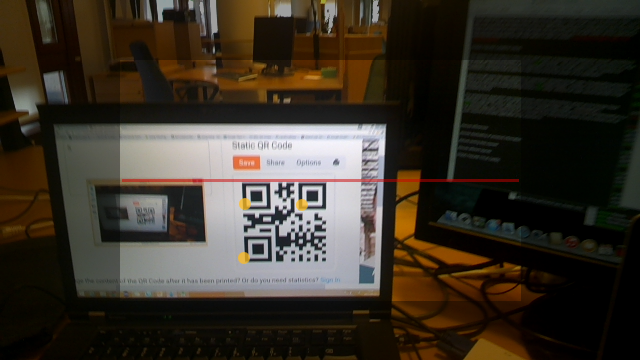
\includegraphics[width=70mm]{images/demo/qrCode}}}
   		 \qquad
		\subfloat[The smartphone application.]{{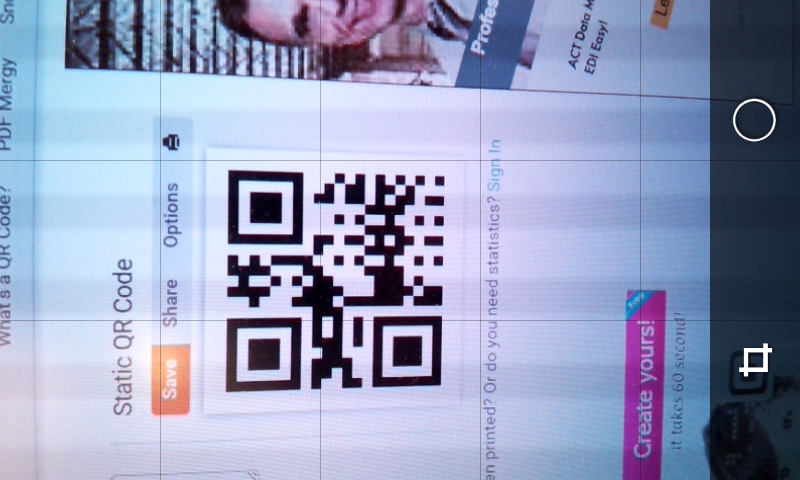
\includegraphics[width=70mm]{images/demo/smartphone/qrCode}}}
   		 \qquad
		\caption{todo bild behöver uppdateras}
		\label{glassDemoQR}
	\end{figure}

The reason for not providing a menu on the start screen was because the application should be simple, easy to use and focus on what is important. Since the the focus of the application is to scan the QR code in order to receive the necessary instructions that is also the main focus of the first screen of the application.

When the QR code has been scanned the application decodes the QR code. The decoding process is done in the same way as described in Section~\ref{subsec:qrcode}. However, the decoding process is handled by the Zebra Crossing (ZXing) library~\cite{zxing}. ZXing is an open source barcode image processing library.

The smartphone application was based directly upon the ZXing library, where as the Google Glass application was based upon a port of the library to Google Glass, called ``BardcodeEye''~\cite{barcodeEye}. The main difference between ZXing and BarcodeEye is the fact that BarcodeEye is a full example application ready to be run, in contrast to the ZXing library which is only a library and as such needs to be attached to a runnable application.

The BarcodeEye application for Google Glass is however a bare bone application, used as an example and introduction as to how ZXing may be implemented in an application for Google Glass. BarcodeEye displayed the decoded information from the QR code and also gave the user the option to search the internet using the information previously decoded from the QR code.

As the QR code was intended to encode only a product ID, and the use the ID to download the instructions, rather than having all of the instructions encoded directly in the QR code the application had to be modified. However, prior to changing where the instructions were coming from the graphical layout of the application was changed. The change of layout was mostly done due to the fact that the application only displayed plain text, not taking in to account for instance a mix of image and text.

However, BarcodeEye also used the deprecated class \texttt{Card}, as seen in Listing~\ref{listingDeprecated}. Instead the application now uses the \texttt{CardBuilder} class, as seen in Listing~\ref{listingRecommended}, as recommended by Google~\cite{googleCard}. The \texttt{CardBuilder} class allows users to input a desired layout style as an argument to the constructor of the \texttt{CardBuilder} class.

\begin{lstlisting}[language=Java, caption={Instancing of the deprecated class Card}, label=listingDeprecated]
Card card = new Card(context);
\end{lstlisting}

\begin{lstlisting}[language=Java, caption={Instancing of the recommended class CardBuilder}, label=listingRecommended]
CardBuilder cardBuilder = new CardBuilder(context, CardBuilder.Layout.TITLE);
\end{lstlisting}

Since the smartphone application also used the ZXing library, but without any pre-existing application, no changes similar to those done to the Google Glass application had to be done for the smartphone application. Instead the smartphone application was built to make use of the ZXing library's functionality, similar to how the ZXing library was integrated in the base Google Glass application.

The Google Glass application and the smartphone application are similar in how they are built up, as seen in Figure~\ref{uml}, which shows a UML diagram over the slide view part of the respective applications.

[TODO UML DIAGRAM ref(uml)]



%discuss differences (classes exclusive to the smartphone application and GG application respectivly)

%discuss downloading of product information
The download process uses the decoded product ID to download information on the specific product. The downloaded information contains the product name, as well as necessary components and instructions for assembling the product. The components and instructions may be represented by text, images or both. 

The way the dpwnload process uses the decoded product ID is by concatinating it with a URl adress, leading to a Web API for a database containing all necessary information regarding the specific product.

The download process also includes creating and initialise an instance of the Products class. The instance contains the name of the product, potentially an image of the product as the product will look when the user is done assembling all the components (the existence of an image is dependent of whether there was an image of the product stored in the database).

The Products class instance will also contain a list of components as well as a list of instructions. Both components and instructions are classes themselves. Similar to the Products class instances of both the Components class and the Instructions class will contain a string and potentially an image. In the case of components the string will contain the name of the component, in contrast to instances of the Instructions class where the string instead will contain the instruction itself.

When the downloaded information is being displayed the first screen the user sees contains the product name as well as an image of the product (if an image has been added to the database). In the example case, lego parts are to be assembled in order to construct the so called ``Space Pirate'', seen in Figure~\ref{glassDemoRaw}.

	\begin{figure}[ht!]
		\centering
		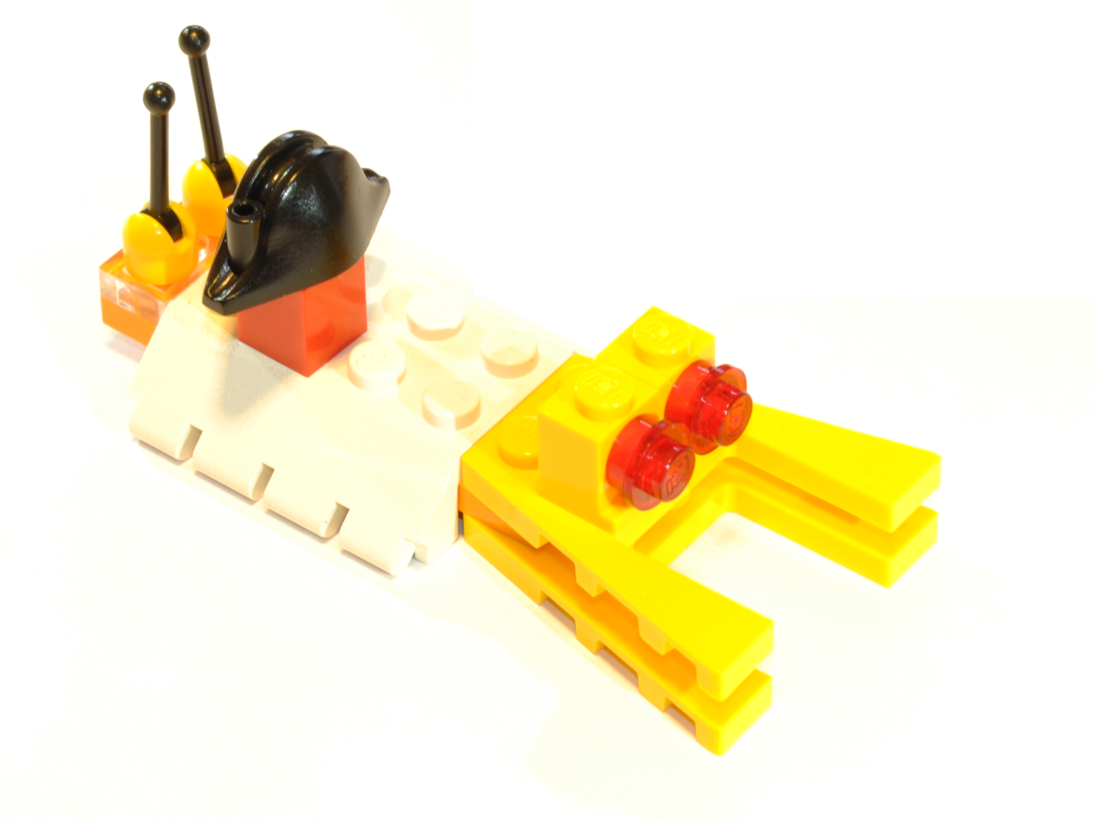
\includegraphics[width=90mm]{images/rawImages/BILD_6}
		\caption{The product.}
		\label{glassDemoRaw}
	\end{figure}

The first information the user sees displayed on screen after the QR code has been scanned and the information has been downloaded is the title page for the Space Pirate product, seen in Figure~{glassDemoTitleCard}.

%	\begin{figure}[H]%ht!]
%		\centering
%		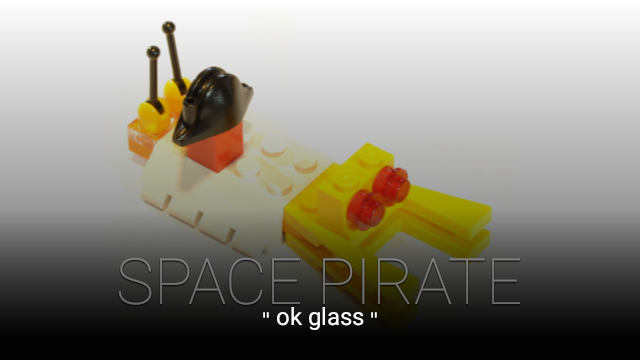
\includegraphics[width=110mm]{images/demo/titleCard}
%		\caption{The title card of the demo application.}
%		\label{glassDemoTitleCard}
%	\end{figure}
	
		\begin{figure}[ht!]
		\centering
    		\subfloat[The Google Glass application]{{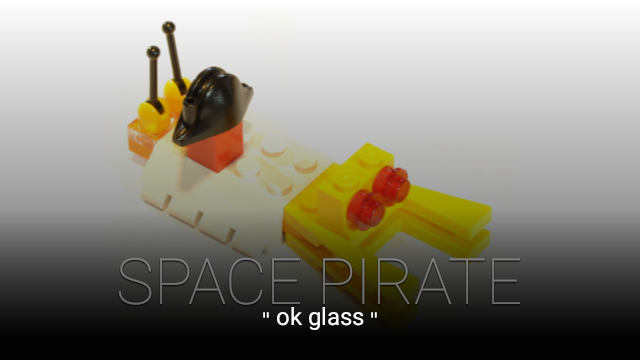
\includegraphics[width=70mm]{images/demo/titleCard}}}
   		 \qquad
		\subfloat[The smartphone application.]{{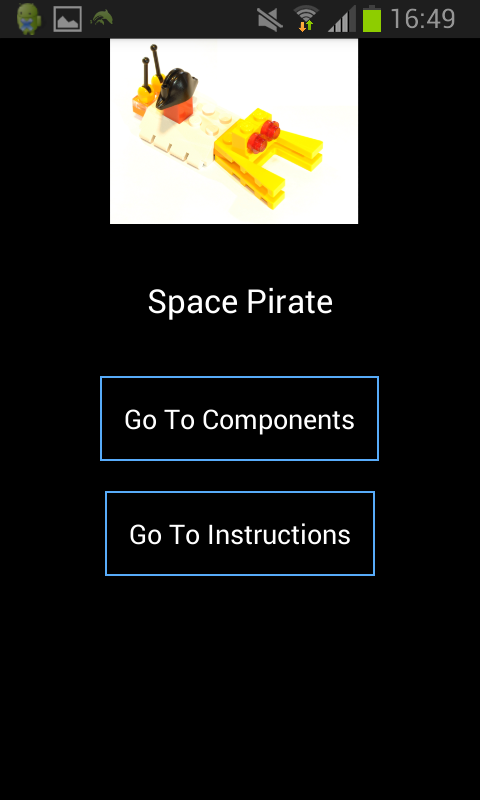
\includegraphics[width=70mm]{images/demo/smartphone/titleCard}}}
   		 \qquad
		\caption{The title card of the demo application.}
		\label{glassDemoTitleCard}
	\end{figure}
	
The nest slide in line after the title slide is the first slide containing information on the components necessary for constructing the specific product. Each component has a separate slide as the component may contain an image in complement to the name of the component. Examples of a component described in only text can been seen in Figure~\ref{flassDemoComponentText} and examples of when the component has been described with both text and image can be seen in Figure~\ref{glassDemoComponentColumn}.
%	\begin{figure}[H]%ht!]
%		\centering
%		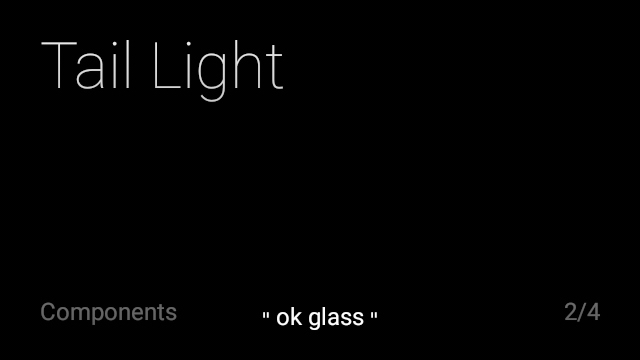
\includegraphics[width=110mm]{images/demo/componentText}
%		\caption{A component slide from the demo application.}
%		\label{glassDemoComponentText}
%	\end{figure}
The card design used for the component slide containing only text, seen in Figure~\ref{glassDemoComponentText}, is the pre defined TEXT layout, used in similar fashion to how the title card design was specified in Listing~\ref{listingRecommended}. A component slide may also contain an image as complement to text. The card design used for the component slide containing both text and image, seen in Figure~\ref{glassDemoComponentColumn} is the pre defined COLUMNS layout, used in similar fashin to how the title card design was specified in Listing~\ref{listingRecommended}

		\begin{figure}[ht!]
		\centering
    		\subfloat[The Google Glass application]{{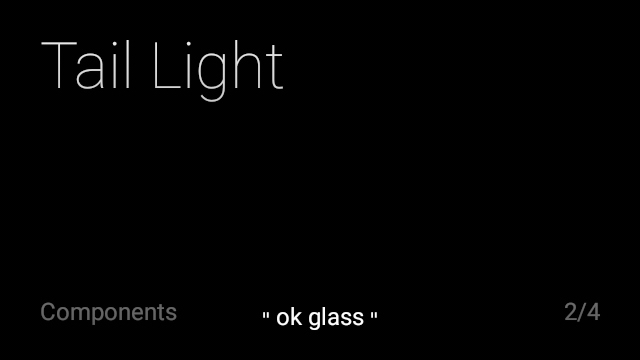
\includegraphics[width=70mm]{images/demo/componentText}}}
   		 \qquad
		\subfloat[The smartphone application.]{{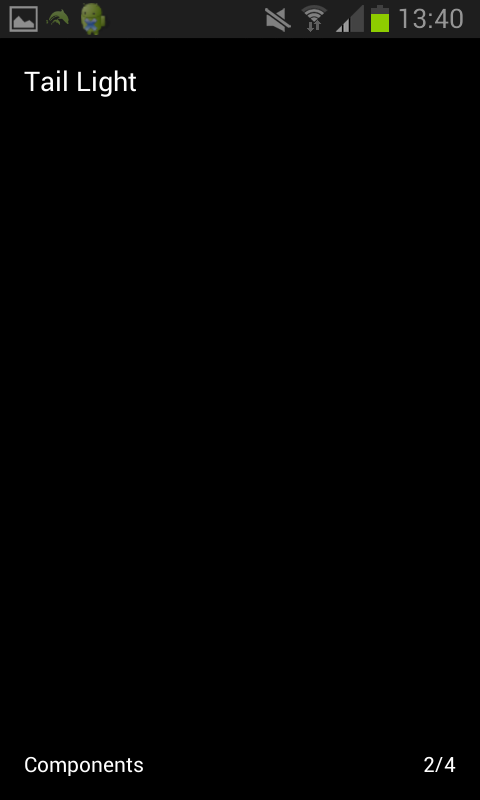
\includegraphics[width=70mm]{images/demo/smartphone/componentText}}}
   		 \qquad
		\caption{A component slide from the demo application.}
		\label{glassDemoComponentText}
	\end{figure}

%	\begin{figure}[H]%ht!]
%		\centering
%		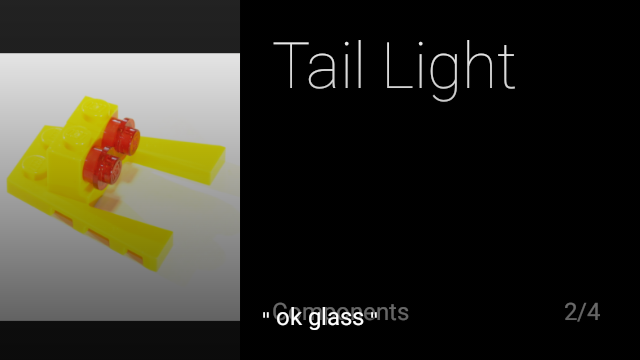
\includegraphics[width=110mm]{images/demo/columnImage}
%		\caption{A component slide from the demo application.}
%		\label{glassDemoComponentColumn}
%	\end{figure}
	
	\begin{figure}[ht!]
		\centering
    		\subfloat[The Google Glass application]{{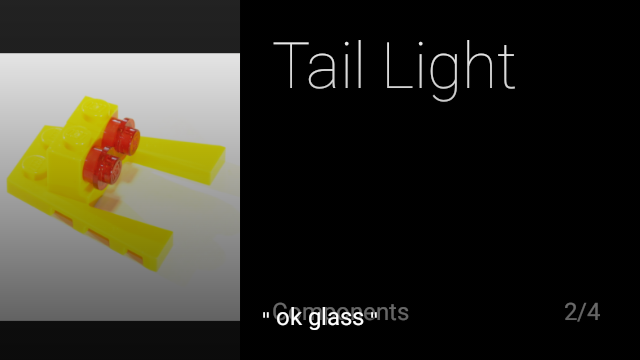
\includegraphics[width=70mm]{images/demo/columnImage}}}
   		 \qquad
		\subfloat[The smartphone application.]{{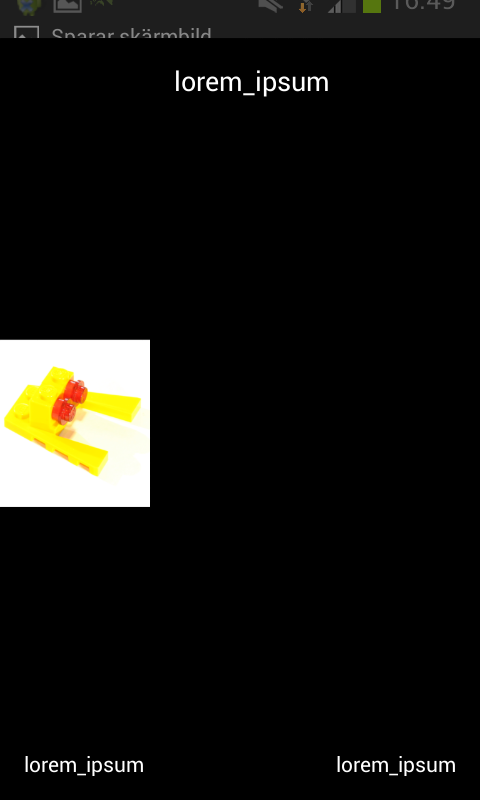
\includegraphics[width=70mm]{images/demo/smartphone/columnImage}}}
   		 \qquad
		\caption{A component slide from the demo application.}
		\label{glassDemoComponentColumn}
	\end{figure}

%	\begin{figure}[H]%ht!]
%		\centering
%		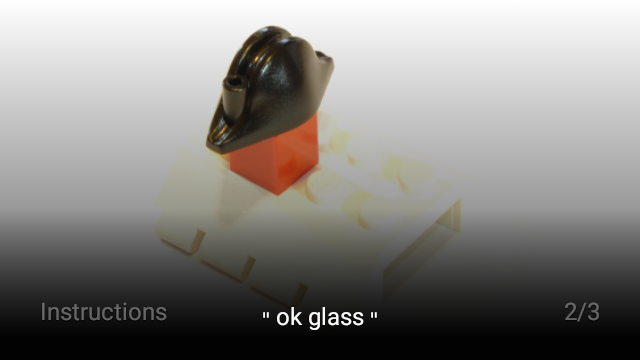
\includegraphics[width=110mm]{images/demo/instructionImage}
%		\caption{An instruction slide from the demo application.}
%		\label{glassDemoInstructionImage}
%	\end{figure}
After all the component slides comes the instruction slides. These slides may also contain either only text or both text and and image, and these layout are specified in the same way as for the component slides. However, an instruction slide may also consist of only an image, and no text at all. The reason for giving an image exclusive layout as a possible card layout for an instruction slide is because an instruction may be best described with an image. Describing the same instruction in text may take up more slides than the image, as the image will only take up one slide. A slide containing only an image and no text will also mean that the image will be scaled biggar than when using both text and an image. As such more detail can be shown and users may get a better understanding for how the components should be assembled.

TODO use demo example to explain why image is better than text Not using image because text takes less space and is faster to download

	\begin{figure}[ht!]
		\centering
    		\subfloat[The Google Glass application]{{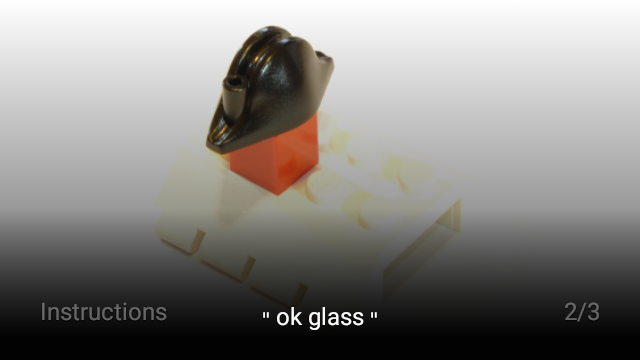
\includegraphics[width=70mm]{images/demo/instructionImage}}}
   		 \qquad
		\subfloat[The smartphone application.]{{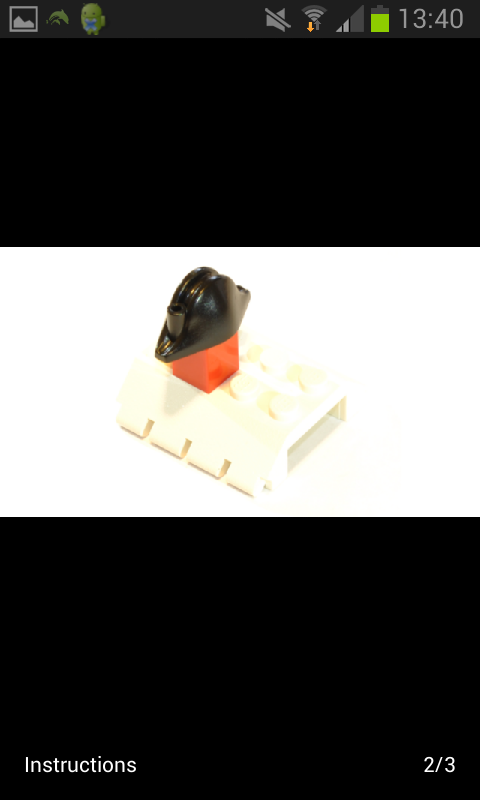
\includegraphics[width=70mm]{images/demo/smartphone/instructionImage}}}
   		 \qquad
		\caption{An instruction slide from the demo application.}
		\label{glassDemoInstructionImage}
	\end{figure}
	
The Google Glass application may be controlled by swiping across the Google Glass touchpad, but the Google Glass application may also be controlled by using voice commands. The voice commands may be used as simple replacement for the touchpad, where users may swipe cards both backwards and forwards. However, using voice commands users may also jump in the application. By for instance saying ``ok glass, show components'' the application jumps to the first component slide, regardless of which slide the user is currently viewing. If the user is currently already viewing the first component slide nothing will happen.
	
	\begin{figure}[ht!]
		\centering
		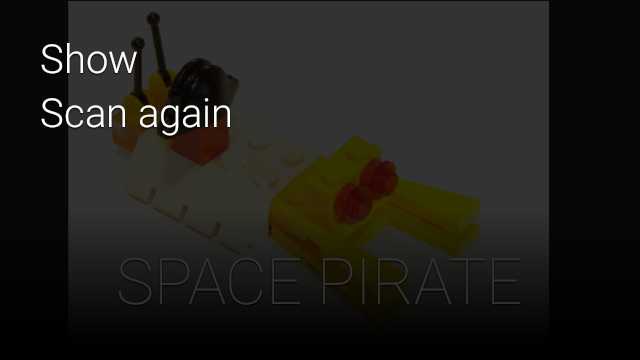
\includegraphics[width=90mm]{images/demo/voiceCommand1}
		\caption{The voice command menu in the demo application.}
		\label{glassDemoVoiceCommand}
	\end{figure}

%discuss sorting into classes

%discuss different layouts